\documentclass[a4paper]{article}
\usepackage[a4paper, margin=1in]{geometry}
% Some basic packages
\usepackage[utf8]{inputenc}
\usepackage[T1]{fontenc}
\usepackage{textcomp}
\usepackage[dutch]{babel}
\usepackage{url}
\usepackage{graphicx}
\usepackage{float}
\usepackage{booktabs}
\usepackage{enumitem}

\pdfminorversion=7

% Don't indent paragraphs, leave some space between them
\usepackage{parskip}

% Hide page number when page is empty
\usepackage{emptypage}
\usepackage{subcaption}
\usepackage{multicol}
\usepackage{xcolor}

% Other font I sometimes use.
% \usepackage{cmbright}

% Math stuff
\usepackage{amsmath, amsfonts, mathtools, amsthm, amssymb}
% Fancy script capitals
\usepackage{mathrsfs}
\usepackage{cancel}
% Bold math
\usepackage{bm}
% Some shortcuts
\newcommand\N{\ensuremath{\mathbb{N}}}
\newcommand\R{\ensuremath{\mathbb{R}}}
\newcommand\Z{\ensuremath{\mathbb{Z}}}
\renewcommand\O{\ensuremath{\emptyset}}
\newcommand\Q{\ensuremath{\mathbb{Q}}}
\newcommand\C{\ensuremath{\mathbb{C}}}

% Easily typeset systems of equations (French package)
\usepackage{systeme}

% Put x \to \infty below \lim
\let\svlim\lim\def\lim{\svlim\limits}

%Make implies and impliedby shorter
\let\implies\Rightarrow
\let\impliedby\Leftarrow
\let\iff\Leftrightarrow
\let\epsilon\varepsilon

% Add \contra symbol to denote contradiction
\usepackage{stmaryrd} % for \lightning
\newcommand\contra{\scalebox{1.5}{$\lightning$}}

% \let\phi\varphi

% Command for short corrections
% Usage: 1+1=\correct{3}{2}

\definecolor{correct}{HTML}{009900}
\newcommand\correct[2]{\ensuremath{\:}{\color{red}{#1}}\ensuremath{\to }{\color{correct}{#2}}\ensuremath{\:}}
\newcommand\green[1]{{\color{correct}{#1}}}

% horizontal rule
\newcommand\hr{
    \noindent\rule[0.5ex]{\linewidth}{0.5pt}
}

% hide parts
\newcommand\hide[1]{}

% si unitx
\usepackage{siunitx}
\sisetup{locale = FR}

% Environments
\makeatother
% For box around Definition, Theorem, \ldots
\usepackage{mdframed}
\mdfsetup{skipabove=1em,skipbelow=0em}
\theoremstyle{definition}
\newmdtheoremenv[nobreak=true]{definitie}{Definitie}
\newmdtheoremenv[nobreak=true]{eigenschap}{Eigenschap}
\newmdtheoremenv[nobreak=true]{gevolg}{Gevolg}
\newmdtheoremenv[nobreak=true]{lemma}{Lemma}
\newmdtheoremenv[nobreak=true]{propositie}{Propositie}
\newmdtheoremenv[nobreak=true]{stelling}{Stelling}
\newmdtheoremenv[nobreak=true]{wet}{Wet}
\newmdtheoremenv[nobreak=true]{postulaat}{Postulaat}
\newmdtheoremenv{conclusie}{Conclusie}
\newmdtheoremenv{toemaatje}{Toemaatje}
\newmdtheoremenv{vermoeden}{Vermoeden}
\newtheorem*{herhaling}{Herhaling}
\newtheorem*{intermezzo}{Intermezzo}
\newtheorem*{notatie}{Notatie}
\newtheorem*{observatie}{Observatie}
\newtheorem*{oef}{Oefening}
\newtheorem*{opmerking}{Opmerking}
\newtheorem*{praktisch}{Praktisch}
\newtheorem*{probleem}{Probleem}
\newtheorem*{terminologie}{Terminologie}
\newtheorem*{toepassing}{Toepassing}
\newtheorem*{uovt}{UOVT}
\newtheorem*{vb}{Voorbeeld}
\newtheorem*{vraag}{Vraag}

\newmdtheoremenv[nobreak=true]{definition}{Definition}
\newtheorem*{eg}{Example}
\newtheorem*{notation}{Notation}
\newtheorem*{previouslyseen}{As previously seen}
\newtheorem*{remark}{Remark}
\newtheorem*{note}{Note}
\newtheorem*{problem}{Problem}
\newtheorem*{observe}{Observe}
\newtheorem*{property}{Property}
\newtheorem*{intuition}{Intuition}
\newmdtheoremenv[nobreak=true]{prop}{Proposition}
\newmdtheoremenv[nobreak=true]{theorem}{Theorem}
\newmdtheoremenv[nobreak=true]{corollary}{Corollary}

% End example and intermezzo environments with a small diamond (just like proof
% environments end with a small square)
\usepackage{etoolbox}
\AtEndEnvironment{vb}{\null\hfill$\diamond$}%
\AtEndEnvironment{intermezzo}{\null\hfill$\diamond$}%
% \AtEndEnvironment{opmerking}{\null\hfill$\diamond$}%

% Fix some spacing
% http://tex.stackexchange.com/questions/22119/how-can-i-change-the-spacing-before-theorems-with-amsthm
\makeatletter
\def\thm@space@setup{%
  \thm@preskip=\parskip \thm@postskip=0pt
}


% Exercise 
% Usage:
% \oefening{5}
% \suboefening{1}
% \suboefening{2}
% \suboefening{3}
% gives
% Oefening 5
%   Oefening 5.1
%   Oefening 5.2
%   Oefening 5.3
\newcommand{\oefening}[1]{%
    \def\@oefening{#1}%
    \subsection*{Oefening #1}
}

\newcommand{\suboefening}[1]{%
    \subsubsection*{Oefening \@oefening.#1}
}


% \lecture starts a new lecture (les in dutch)
%
% Usage:
% \lecture{1}{di 12 feb 2019 16:00}{Inleiding}
%
% This adds a section heading with the number / title of the lecture and a
% margin paragraph with the date.

% I use \dateparts here to hide the year (2019). This way, I can easily parse
% the date of each lecture unambiguously while still having a human-friendly
% short format printed to the pdf.

\usepackage{xifthen}
\def\testdateparts#1{\dateparts#1\relax}
\def\dateparts#1 #2 #3 #4 #5\relax{
    \marginpar{\small\textsf{\mbox{#1 #2 #3 #5}}}
}

\def\@lecture{}%
\newcommand{\lecture}[3]{
    \ifthenelse{\isempty{#3}}{%
        \def\@lecture{Lecture #1}%
    }{%
        \def\@lecture{Lecture #1: #3}%
    }%
    \subsection*{\@lecture}
    \marginpar{\small\textsf{\mbox{#2}}}
}



% These are the fancy headers
\usepackage{fancyhdr}
\pagestyle{fancy}

% LE: left even
% RO: right odd
% CE, CO: center even, center odd
% My name for when I print my lecture notes to use for an open book exam.
% \fancyhead[LE,RO]{Gilles Castel}

\fancyhead[RO,LE]{\@lecture} % Right odd,  Left even
\fancyhead[RE,LO]{}          % Right even, Left odd

\fancyfoot[RO,LE]{\thepage}  % Right odd,  Left even
\fancyfoot[RE,LO]{}          % Right even, Left odd
\fancyfoot[C]{\leftmark}     % Center

\makeatother




% Todonotes and inline notes in fancy boxes
\usepackage{todonotes}
\usepackage{tcolorbox}

% Make boxes breakable
\tcbuselibrary{breakable}

% Verbetering is correction in Dutch
% Usage: 
% \begin{verbetering}
%     Lorem ipsum dolor sit amet, consetetur sadipscing elitr, sed diam nonumy eirmod
%     tempor invidunt ut labore et dolore magna aliquyam erat, sed diam voluptua. At
%     vero eos et accusam et justo duo dolores et ea rebum. Stet clita kasd gubergren,
%     no sea takimata sanctus est Lorem ipsum dolor sit amet.
% \end{verbetering}
\newenvironment{verbetering}{\begin{tcolorbox}[
    arc=0mm,
    colback=white,
    colframe=green!60!black,
    title=Opmerking,
    fonttitle=\sffamily,
    breakable
]}{\end{tcolorbox}}

% Noot is note in Dutch. Same as 'verbetering' but color of box is different
\newenvironment{noot}[1]{\begin{tcolorbox}[
    arc=0mm,
    colback=white,
    colframe=white!60!black,
    title=#1,
    fonttitle=\sffamily,
    breakable
]}{\end{tcolorbox}}




% Figure support as explained in my blog post.
\usepackage{import}
\usepackage{xifthen}
\usepackage{pdfpages}
\usepackage{transparent}
\newcommand{\incfig}[1]{%
    \def\svgwidth{\columnwidth}
    \import{./figures/}{#1.pdf_tex}
}

% Fix some stuff
% %http://tex.stackexchange.com/questions/76273/multiple-pdfs-with-page-group-included-in-a-single-page-warning
\pdfsuppresswarningpagegroup=1

\title{\Huge{Homework 6}}
\author{\huge{Daniel Yu}}
\date{October 19,2024}

\pdfsuppresswarningpagegroup=1

\begin{document}
\maketitle
\newpage% or \cleardoublepage
% \pdfbookmark[<level>]{<title>}{<dest>}
\pagebreak

\begin{enumerate}
  \item There are two jars in front of you and a total $n$ balls divided among them. Every minute, you pick a ball uniformly at random, and move it to another jar. Let $X_n$ denote the number of balls in the first jar. Argue that  $\{X_n\} $ is a markov chain and calculate its transition probabilities. 
    \begin{proof}
    Consider the markov chain with states $\{S_0, S_1, \ldots, S_n \}$. The different states represent the differen t numbers of balls that could belong in the first jar at each timestep $X_n$. Thus, for state  $S_i$, the transition probability to  $S_{i+1}$ would be $\frac{n-i}{n}$ the probability a ball is chosen from the second jar and moved to the first jar. Similarly, the transition probability from  $S_i$ to  $S_{i-1}$ would be $\frac{i}{n}$ the probability a ball is moved from the first jar to the second jar. This would be for all states $S_1, \ldots, S_n$ and then for  $S_0$, the transition probability would be $1$ to $S_1$ and  $S_n$ the transition probability would be $1$ to  $S_{n-1}$. \\

    $\{X_n\} $ is a markov chain because at every time $X_n$,  
    \begin{align*}
      P[X_n = S_j \mid X_{n-1} = S_{j_{n-1}}, \ldots, X_{0} = S_{j_{0}}] &= P[X_n = S_j \mid X_{n-1} = S_{j_{n-1}}]\\ &= \begin{cases}
      \frac{n-j_{n-1}}{n}, S_{j} = S_{j_{n-1}} + 1 \\
      \frac{j_{n-1}}{n}, S_{j} = S_{j_{n-1}} - 1 \\
      0, \text{ otherwise}
    \end{cases}
    .\end{align*} By construction, the probability of the next state is only dependent on the previous state. Thus, since it's a stochastic process (since $X_k$ are timesteps) with the above property, then  $\{X_n\} $ is a markov chain. 
  \end{proof}
\item  Let $Y_n$ be a time homogenous markov chain with states  $\{1,2,3\}$. The transition probabilities for $Y_n$ are summarized in the matrix below where  $P_{i,j} = P[Y_1 = j \mid  Y_0 = i]$. 
  \[
    P = \begin{pmatrix}
\frac{1}{2} & \frac{1}{3} & \frac{1}{6} \\
\frac{1}{3} & 0 & \frac{2}{3} \\
\frac{1}{2} & \frac{1}{2} & 0
\end{pmatrix}
  .\] 
  If $P[Y_0=1] = P[Y_0 =3] = \frac{1}{2}$, compute $E[Y_3]$. 
  \begin{proof}
   \[
   P^3 = \begin{pmatrix}
0.4583 & 0.3009 & 0.2407 \\
0.4259 & 0.1944 & 0.3796 \\
0.4722 & 0.3472 & 0.1806
\end{pmatrix}, V_0 = \begin{pmatrix} 
\frac{1}{2}\\
0 \\
\frac{1}{2}
\end{pmatrix} 
   .\] 
   We know that:
   \begin{align*}
     E[Y_3] &= \sum_{k=1}^{3} k \cdot P[Y_3 = k] \\
            &= \sum_{k=1}^{3} k (\sum_{i=1}^{3} P[Y_0=i] \cdot P[Y_3=k\mid Y_0 = i])\\
            &= \sum_{k=1}^{3} k \left( P^{3} \cdot v_0 \right)_{k}  \\
            &=  \sum_{k=1}^{3} k  \begin{pmatrix}
0.3495 \\
0.4027 \\
0.3264
\end{pmatrix}_{k} \\
            &=  \begin{pmatrix} 1 \\ 2 \\ 3 \end{pmatrix}^{T} \cdot \begin{pmatrix}
0.3495 \\
0.4027 \\
0.3264
\end{pmatrix} \\
                                      &= 2.1341 
   .\end{align*}
  \end{proof}
  \item Suppose that P is transition matrix for some finite-state Markov chain. Suppose that there
exists an integer $r \geq 1$ such that every entry in $P^{r}$ is strictly positive. Argue that, for any $n \geq r$,
every entry of P n is also strictly positive.

\begin{proof}
 Since $P$ is a transition matrix, then we know that every entry is non-negative. Furthermore,  $\forall i, \sum_{j} P_{i,j} = 1$, the matrix must be row stochastic. If there exists an integer $r \geq 1$ such that every matrix entry in  $P^{r}$ is also strictly positive, then this means that:
 \[
 P^{r} = P \times P \times P \ldots \times P
 .\] 
 is strictly positive as well. Suppose that $P$ had a column of all zeros. Let this column be the  $i$th column. Then, since whatever row multipled by that column results in 0,  $\forall j, P^{2}_{i,j} = 0$.
\[
\begin{pmatrix}
\cdot & \cdot & 0 & \cdot & \cdot & \cdot \\
\cdot & \cdot & 0 & \cdot & \cdot & \cdot \\
\cdot & \cdot & 0 & \cdot & \cdot & \cdot \\
\vdots & \vdots & \vdots & \vdots & \vdots & \vdots \\
\cdot & \cdot & 0 & \cdot & \cdot & \cdot \\
\end{pmatrix} \times 
\begin{pmatrix}
\cdot & \cdot & 0 & \cdot & \cdot & \cdot \\
\cdot & \cdot & 0 & \cdot & \cdot & \cdot \\
\cdot & \cdot & 0 & \cdot & \cdot & \cdot \\
\vdots & \vdots & \vdots & \vdots & \vdots & \vdots \\
\cdot & \cdot & 0 & \cdot & \cdot & \cdot \\
\end{pmatrix}
= 
\begin{pmatrix}
\cdot & \cdot & 0 & \cdot & \cdot & \cdot \\
\cdot & \cdot & 0 & \cdot & \cdot & \cdot \\
\cdot & \cdot & 0 & \cdot & \cdot & \cdot \\
\vdots & \vdots & \vdots & \vdots & \vdots & \vdots \\
\cdot & \cdot & 0 & \cdot & \cdot & \cdot \\
\end{pmatrix}
.\]  
Thus, $\forall j, P^{r}_{i,j} = P\times P \times P \ldots \times P = 0$. This violates our assumption that $P^{r}$ has strictly positive entries. So there, can't be a column of all zeros. Now let's use induction, we assume that $P^{r}$ is strictly positive, then $P^{r+1} = P^{r} \cdot P$ must also be strictly positive, because every row of $P^{r}$ has every value as non-zero and $P$ must have every column containing at least one non-zero value. So, $P^{r+1}_{i,j} > 0$.  By induction, this hold for $n \geq r$!
\end{proof}
\item We have a Markov chain on five states, numbered 1, 2, 3, 4, 5. At each state, the Markov chain
is equally likely to go to any state whose number is greater than or equal to itself. The state 5 is
an absorbing state. Let T be the first time of absorption — that is, $T = \min\{t ∶ X_t = 5\}$. Find the
expected value of T , if $X_0 = 1$. 

\begin{proof}
  We first must calculate $N = (I-Q)^{-1}$. Since $5$ is the only absorbing state, then $Q$ consists of the states  $1,2,3,4$ and the connections between them and  $I$ is just  $1$.
 
\begin{figure}[h]
  \centering
  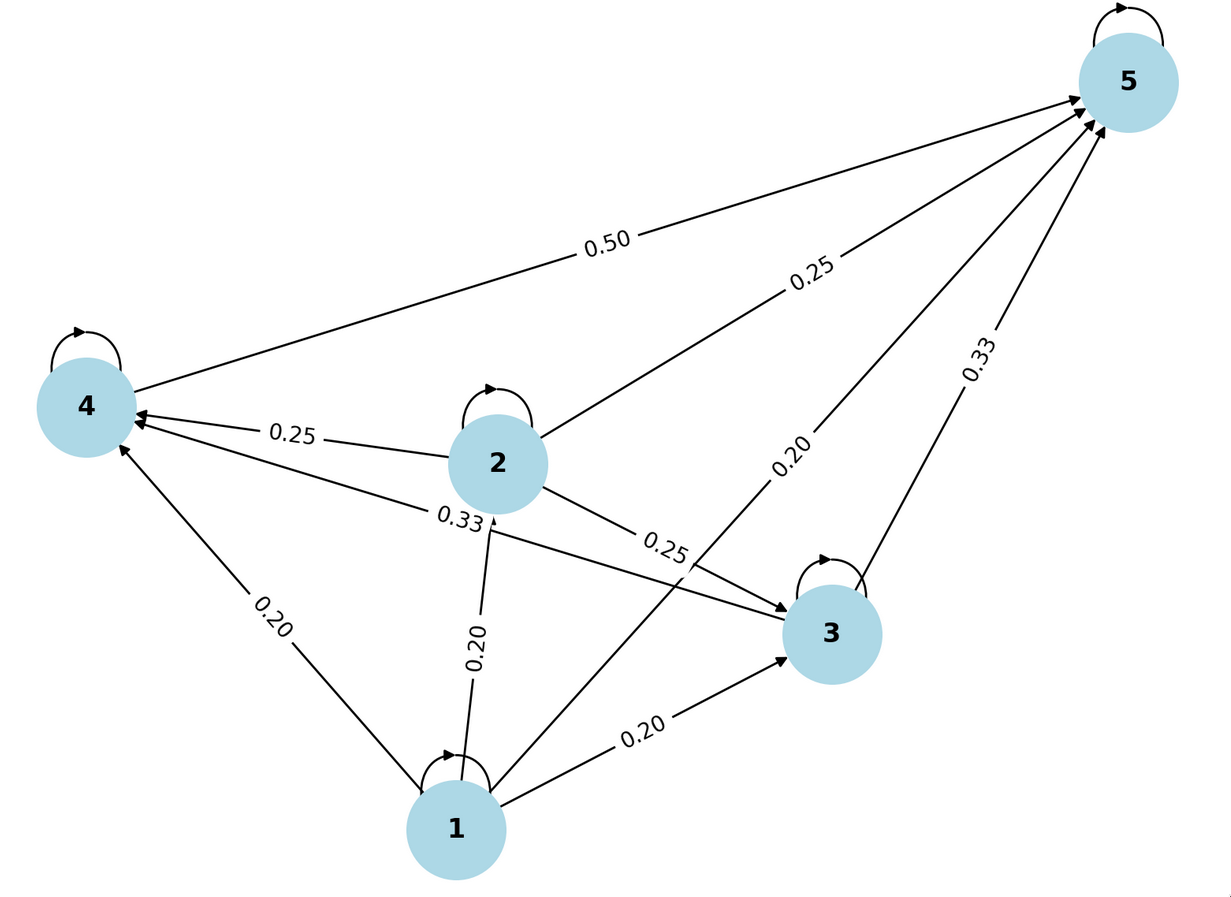
\includegraphics[width=0.8\textwidth]{assets/markov_chain_absorption.png}
  \caption{Problem 4 Markov Chain}
  \label{fig:markov_chain_absorption}
\end{figure}
Thus, we have the following matrix
\[
\begin{pmatrix}
0.20 & 0.20 & 0.20 & 0.20 & 0.20 \\
0.00 & 0.25 & 0.25 & 0.25 & 0.25 \\
0.00 & 0.00 & 0.33 & 0.33 & 0.33 \\
0.00 & 0.00 & 0.00 & 0.50 & 0.50 \\
0.00 & 0.00 & 0.00 & 0.00 & 1.00 \\
\end{pmatrix}
.\]
Then,
\[
N =  (\begin{pmatrix}
1 & 0 & 0 & 0 \\
0 & 1 & 0 & 0 \\
0 & 0 & 1 & 0 \\
0 & 0 & 0 & 1 
\end{pmatrix}  - \begin{pmatrix}
0.20 & 0.20 & 0.20 & 0.20 \\
0.00 & 0.25 & 0.25 & 0.25 \\
0.00 & 0.00 & 0.33 & 0.33 \\
0.00 & 0.00 & 0.00 & 0.50 
\end{pmatrix})^{-1} =  \begin{pmatrix}
1.25 & 0.3333 & 0.4975 & 0.9950 \\
0.00 & 1.3333 & 0.4975 & 0.9950 \\
0.00 & 0.00 & 1.4925 & 0.9851 \\
0.00 & 0.00 & 0.00 & 2.00 \\
\end{pmatrix}
.\] 
We know that 
\[
  E[T \mid X_0 = 1] = \sum_{j=1}^{n} (N)_{1,j} = (N \cdot \vec{1})_{1} = 3.076
.\] 
\end{proof}
  \item In tennis, a player must win by at least two points. If the players are tied (and both have won at
least three points), deuce is reached. If one player is leading by one, they have advantage. Assume
that player one has advantage, but has a probability of 2/5 of winning any given point; further
assume that the outcomes of different points are independent. What is the probability that player
one wins the game?
\begin{proof}
We are given a game of tennis where Player 1 has the advantage, i.e. player 1 and 2 have score both at least  $3$ points and Player 1 is one point ahead. The probability of Player 1 winning a point is $\frac{2}{5}$ and the probability of Player  losing a point is $\frac{3}{5}$. Naturally, if either player has a lead of 2 points, then they win the game. Thus, we can construct the following markov chain which represents the point differential between player 1 and 2. Since we are given that Player 1 has advantage, we don't have to consider the previous points, only that the intial state is player  $1$ has 1 point ahead.
\begin{figure}[h]
  \centering
  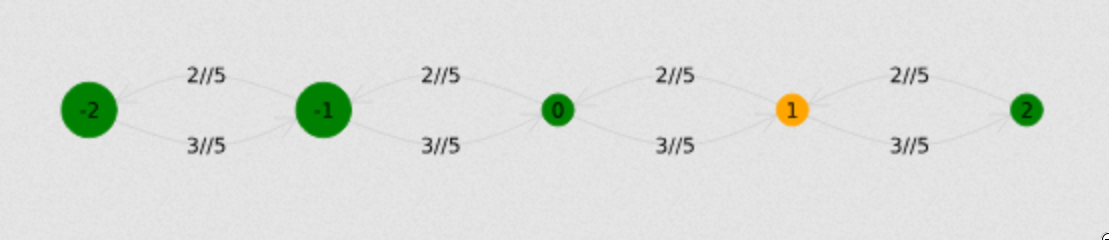
\includegraphics[width=0.8\textwidth]{assets/markov_chain_tennis_problem.png}
  \caption{Problem 5 Graph}
  \label{fig:markov_chain_tennis_problem}
\end{figure}
Denote the probability that Player 1 then wins from advantage as $W_A$ and wins from Deuce as  $W_D$ and wins from down 1 as $W_L$
\begin{align}
  W_A &= \frac{2}{5} + \frac{3}{5} W_D \\
  W_D &= \frac{2}{5} W_A + \frac{3}{5}W_L \\
  W_L &= \frac{2}{5} W_D + \frac{3}{5} \cdot 0 
.\end{align}
Substitute $W_L$ into  $W_D$
 \begin{align*}
  W_D &= \frac{2}{5} W_A + \frac{3}{5}W_L \\
      &= \frac{2}{5} W_A + \frac{3}{5}\left( \frac{2}{5} W_D  \right) \\
  \frac{19}{25} W_D  &= \frac{2}{5}W_A  \\
  W_D &= \frac{10}{19}W_A
.\end{align*}
Substitute into $W_A$:
\begin{align*}
  W_A &= \frac{2}{5} + \frac{3}{5} W_D \\
      &= \frac{2}{5} + \frac{3}{5} \left( \frac{10}{19} W_A \right) \\
      &= \frac{2}{5} + \frac{6}{19} W_A \\
      &= \frac{38}{95} + \frac{30}{95} W_A\\
   \frac{65}{95} W_A &= \frac{38}{95} \\
                     &= \frac{38}{65}
.\end{align*}
\end{proof}
\end{enumerate}
\end{document}
